\documentclass[12pt]{article}
\usepackage[a4paper,margin=0.6in]{geometry}
\usepackage{titlesec}
\usepackage{graphicx}
\usepackage{enumitem}
\usepackage{caption}
\usepackage{hyperref}
\titleformat{\section}{\Large\bfseries}{\thesection}{1em}{}
\title{\textbf{{\Huge{EcoSync 8X}\\ \Large{USER MANUAL}}}}
\author{}
\date{}

\begin{document}

\maketitle
\begin{figure}[h]
    \centering
    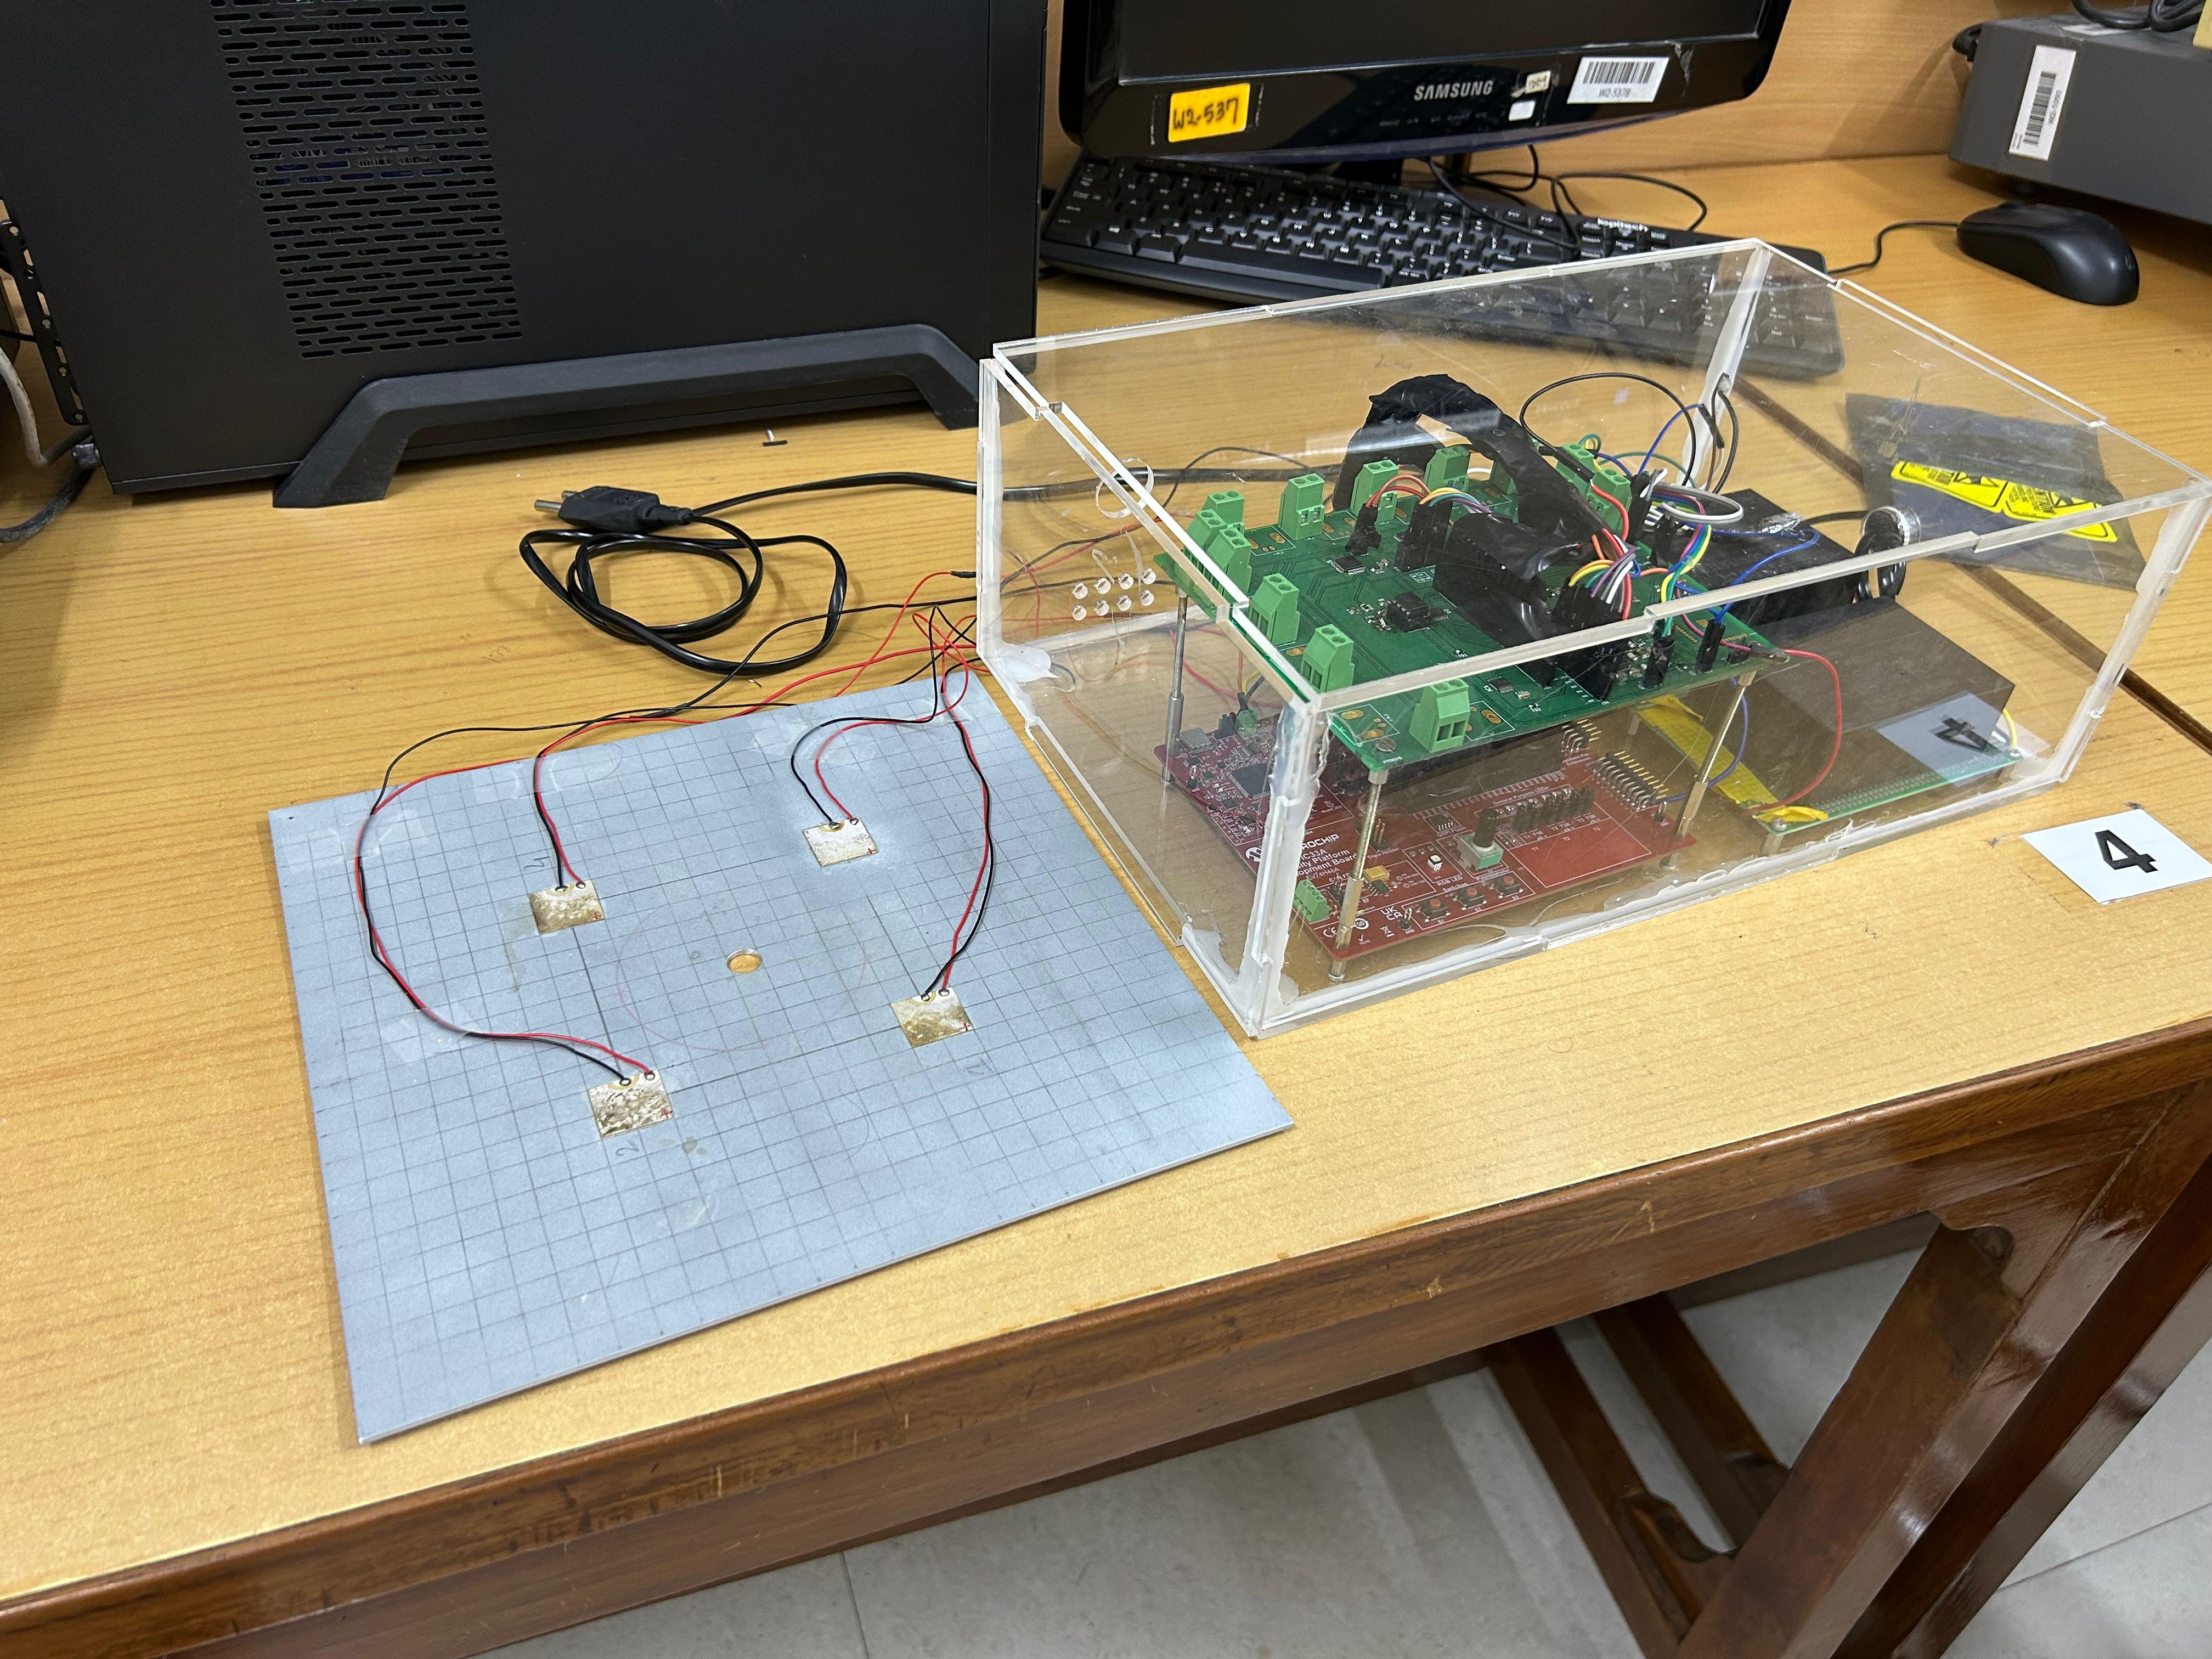
\includegraphics[width=0.65\linewidth]{OV_main_1.jpg}
    \caption*{dsPIC33A microcontroller based ultrasonic guided wave structural health monitoring system}
\end{figure}
\section*{Detailed Setup Instructions}

\begin{enumerate}[label=\textbf{Step \arabic*:}, leftmargin=2.5em]

\item \textbf{Connect piezoelectric sensors to the plate in an organized manner.}
\\$\bullet$ Mount each piezoelectric sensor firmly on the surface of the test plate according to your sensor layout plan.\\ $\bullet$ Ensure consistent spacing if required and align sensors to match the coordinate reference for accurate mapping.\\ Label or note the position of each sensor for easy identification when assigning them as transmitters or receivers later in the application.\\$\bullet$ Use strong adhesive or proper fixtures to ensure good mechanical coupling between the sensors and the plate for efficient wave transmission and reception.

\item \textbf{Connect the plug to a 220V, 15A supply socket.} \\
$\bullet$Locate a stable and grounded 220-volt AC power outlet rated for 15 amps.\\$\bullet$ Connect the system's power plug securely to the socket.\\ $\bullet$Ensure there’s no physical damage to the plug or socket, and avoid using loose or multi-plug extensions that could cause overheating or voltage drops.\\$\bullet$ This power supply will energize the signal generation and data acquisition units within the system.

\item \textbf{Connect your computer to the Wi-Fi module.}\\$\bullet$ Turn on the Wi-Fi of your computer and connect to the access point broadcast by the Wi-Fi module connected to the control box.\\$\bullet$ No internet connection is needed; this local connection is for direct data communication between your system and the application.\\$\bullet$ Ensure that that your computer's firewall or antivirus software does not block the communication port used by the application.

\item \textbf{Open your application and enter which piezoelectric sensors you want to use as transmitters and receivers.} \\
$\bullet$Launch the custom SHM (Structural Health Monitoring) software on your computer.\\$\bullet$ Once it detects the connected Wi-Fi module, the user interface will allow you to assign roles to each sensor (Tx/Rx).\\$\bullet$ Transmitters send the ultrasonic signal, while receivers capture the reflected waves that interact with potential defects.\\$\bullet$ Select sensors strategically to cover the full structure or specific areas of interest. This configuration directly affects the resolution and accuracy of damage detection.\\

\item \textbf{Data will be received over Wi-Fi after some time. Press the orange button to get the DI Map.} \\
$\bullet$After transmission, the system will gather signal responses from the receivers and process them onboard or via your computer. Data is sent wirelessly back to the computer and might take a few seconds depending on the number of sensors and sampling rate.\\$\bullet$ Once data is received and processed, click the \textbf{orange button} on the application interface to generate the \textbf{Damage Index (DI) Map}. This map visually represents possible damage areas based on signal attenuation, scattering, or time delay.

\end{enumerate}

\section*{Precautions}

\begin{itemize}
    \item \textbf{Do not touch the wiring or control box when plugged in to avoid electric shock.} \\
    High-voltage components inside the control box could pose a risk of shock. Make all sensor connections and hardware checks \textit{before} plugging the system in. If adjustment is needed while powered, use insulated tools and gloves, or power off first.

    \item \textbf{Handle the control box with care during transportation.} \\
    The control box contains delicate electronics such as amplifiers, ADCs, microcontrollers, or signal conditioning boards. Use padding or a protective case during transport to prevent mechanical damage. Avoid placing heavy objects on top of the box or exposing it to moisture or extreme heat.
\end{itemize}

\end{document}
